\documentclass[11pt, a4paper, twoside]{article}

% Versión 1.er cuat 2021 Víctor Bettachini < vbettachini@unlam.edu.ar >

\usepackage[T1]{fontenc}
\usepackage[utf8]{inputenc}

% \usepackage[spanish, es-tabla]{babel}
\def\spanishoptions{argentina} % Was macht dass?
% \usepackage{babelbib}
% \selectbiblanguage{spanish}
% \addto\shorthandsspanish{\spanishdeactivate{~<>}}

\usepackage{graphicx}
\graphicspath{{./figuras/}{../LaTeX/}{../figurasLaTeX/}}
% \usepackage{float}

\usepackage[arrowdel]{physics}
\newcommand{\pvec}[1]{\vec{#1}\mkern2mu\vphantom{#1}}
% \usepackage{units}
\usepackage[separate-uncertainty= true, multi-part-units= single, range-units= single, range-phrase= {~a~}, locale= FR]{siunitx}
\usepackage{isotope} % $\isotope[A][Z]{X}\to\isotope[A-4][Z-2]{Y}+\isotope[4][2]{\alpha}

\usepackage{tasks}
\usepackage[inline]{enumitem}
% \usepackage{enumerate}

\usepackage{hyperref}

% \usepackage{amsmath}
% \usepackage{amstext}
% \usepackage{amssymb}

\usepackage{tikz}
\usepackage{tikz-3dplot}
\usepackage{tikz-dimline}
\usetikzlibrary{calc}
% \usetikzlibrary{math}
\usetikzlibrary{arrows.meta}
\usetikzlibrary{snakes}
\usetikzlibrary{decorations}
\usetikzlibrary{decorations.pathmorphing}
\usetikzlibrary{patterns}

\usepackage[hmargin=1cm,vmargin=3cm, top= 0.75cm,nohead]{geometry}

\usepackage{lastpage}
\usepackage{fancyhdr}
\pagestyle{fancyplain}
\fancyhf{}
\setlength\headheight{28.7pt} 
\fancyhead[LE, LO]{\textbf{Computational Analytical Mechanics} }
% \fancyhead[LE, LO]{\textbf{Mecánica General} }
\fancyhead[RE, RO]{\href{https://ingenieria.unlam.edu.ar/}{$\vcenter{\hbox{
\includegraphics[height=1cm]{../../../../figurasLaTeX/ambos.pdf}}}$}}  %edg fix path
\fancyfoot{\href{https://creativecommons.org/licenses/by-nc-sa/4.0/deed.es_ES}{$\vcenter{\hbox{
\includegraphics[height=0.4cm]{../../../../figurasLaTeX/by-nc-sa_80x15.pdf}}}$} \href{https://ingenieria.unlam.edu.ar/}{DIIT - UNLaM}}  %edg fix path
\fancyfoot[C]{ {\tiny Updated on \today} }
\fancyfoot[RO, LE]{Pág. \thepage/\pageref{LastPage}}
\renewcommand{\headrulewidth}{0pt}
\renewcommand{\footrulewidth}{0pt}



\begin{document}

\begin{center}
  % \textsc{\large Mecánica general}\\
  \textsc{\large Coordenadas generalizadas | Ligaduras | Energías cinética y potencial}
\end{center}
\noindent
Los problemas marcados con (*) tienen alguna dificultad adicional, no dude en consultar.

\begin{enumerate}

\item
	\begin{minipage}[t][5cm]{0.7\textwidth}
		\textbf{Péndulo con punto de suspensión libre} [Landau \S5 ej. 2]\\
		La partícula de masa \(m_2\) pende de una barra rígida de longitud \(\ell\) de masa despreciable.
		En su otro extremo hay un dispositivo de masa \(m_1\) enhebrado en una barra rígida horizontal y que se mueve libremente a lo largo de su eje \(\hat{x}\).
		El dispositivo permite que la barra que pende de él forme con la vertical cualquier ángulo \(\varphi\). 
		\begin{enumerate}
			\item Escriba la energía cinética, \(T\) y potencial, \(V\), en función de las coordenadas generalizadas sugeridas por las figura.
			\item Verifique que al fijar la masa \(m_1\) recupera las expresiones de \(T\) y \(V\) de un péndulo ideal.
		\end{enumerate}
	\end{minipage}
	\begin{minipage}[c][1cm][t]{0.3\textwidth}
		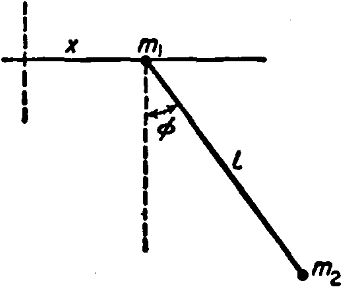
\includegraphics[width=0.75\textwidth]{figures/landauS52_fig2.png}
	\end{minipage}



\item
	\begin{minipage}[t][4cm]{0.7\textwidth}
		\textbf{Péndulo doble} [Landau \S5 ej. 1]\\
		Una barra rígida de longitud \(\ell_1\) tiene una masa despreciable respecto a la de la partícula de masa \(m_1\) fija a su extremo.
		A su vez de esta última pende otra barra rígida, de longitud \(\ell_2\) que en su extremo tiene otra partícula de masa \(m_2\), también mucho mayor que aquella de la barra.
		\begin{enumerate}
			\item Escriba la energía cinética, \(T\) y potencial, \(V\), en función de las coordenadas generalizadas sugeridas por las figura.
			\item Verifique que recupera \(T\) y \(V\) de un péndulo simple si establece \(m_1=0\), \(\varphi_1 = \varphi_2 = \varphi\) y \(\ell_1 = \ell_2 = \frac{\ell}{2}\).
		\end{enumerate}
		% Ayuda: \( \cos(\alpha \pm \beta) = \cos{ \alpha} \cos{ \beta \mp \sin \alpha} \sin{ \beta } \)
	\end{minipage}
	\begin{minipage}[c][0.5cm][t]{0.3\textwidth}
		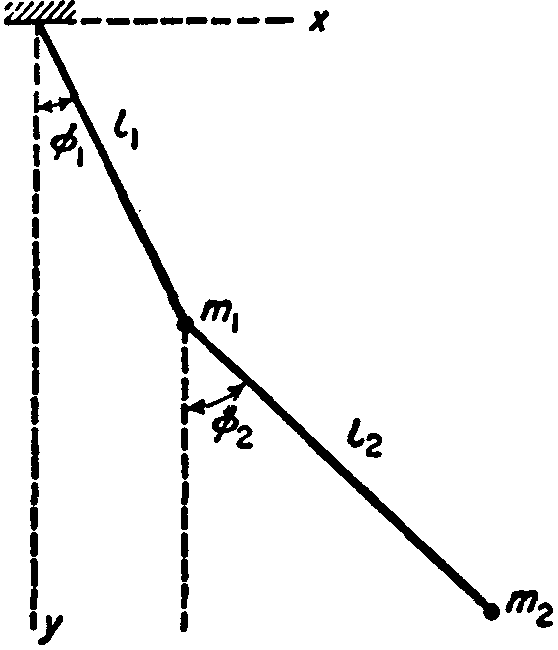
\includegraphics[width=0.75\textwidth]{figures/landauS52_fig1.png}
	\end{minipage}



\item
	\begin{minipage}[t][7.1cm]{0.5\textwidth}
		(*) \textbf{Péndulo con punto de suspensión en rotación} [Marion (e) ex. 7.5] [Landau \S5 ej. 3]\\

		Una partícula de masa \(m\) pende de una barra rígida de longitud \(b\).
		El punto de suspensión engarzado en un aro de radio \(a\) dispuesto verticalmente rota respecta a su centro con una frecuencia \(\omega\) constante.
		Se asume que todas las posiciones se encuentran en un único plano bidimensional y que la masa de la barra rígida tiene masa despreciable frente a \(m\).

		Calcule la energía cinética, \(T\) y potencial, \(V\) de la partícula con masa \(m\).\end{minipage}
	\begin{minipage}[c][3cm][t]{0.5\textwidth}
		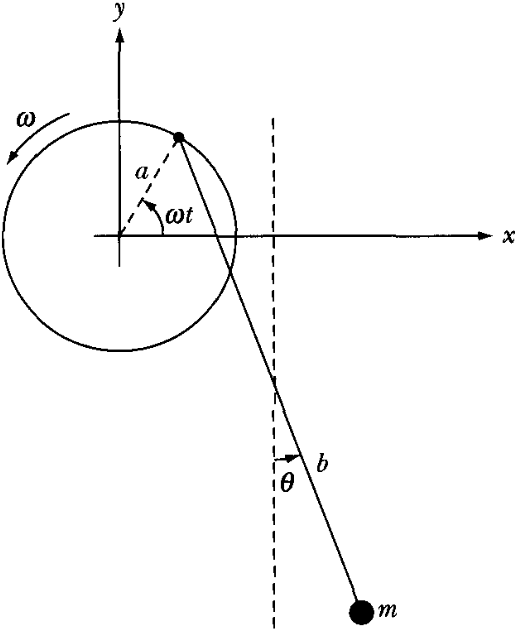
\includegraphics[width=0.75\textwidth]{figures/marion_fig7_3.png}
		% \includegraphics[width=0.75\textwidth]{landauS52_fig3.png}
	\end{minipage}



\item
	\begin{minipage}[t][4.5cm]{0.65\textwidth}
		(*) \textbf{Pesas acopladas rotando en torno a eje} [Landau \S5 ej. 4]\\

		La partícula con \(m_2\) se desplaza sobre un eje vertical, y todo el sistema gira con una velocidad angular constante \(\Omega\) en torno a ese eje.
		Dicha partícula está unida por barras de longitud \(a\) y masa despecible a otras dos de masa \(m_1\) que a su vez pendend de sendas barras idénticas del punto fijo \(A\) que describen un ángulo de apertura respecto al eje \(\theta\) que es variable.

			Calcule la energía cinética para cada una de las tres masas y exprese en la forma más compacta posible la del sistema en su conjunto.
	\end{minipage}
	\begin{minipage}[c][1cm][t]{0.35\textwidth}
		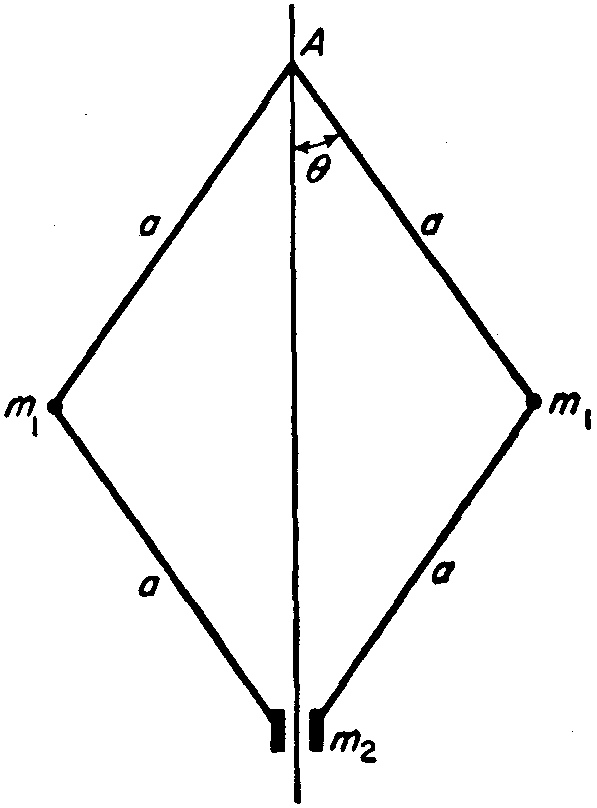
\includegraphics[width=0.75\textwidth]{figures/landauS52_fig4.png}
	\end{minipage}



\end{enumerate}
\end{document}
